\subsection{Problem definition}
We address natural language inference (NLI) and its special case of paraphrasing (PP).
Models train on datasets like MNLI for NLI or QQP for PP
are prune to learn some syntactic heuristics as it 
is shown in \newcite{linzen2019right,zhang-etal-2019-paws}.
The main heuristics is the word overlap between hypothesis and premis. \newcite{naik2018stress} study some misclassified examples and find that word overlap is the major reason (29\% of cases). For NLI, there is high correlation between large word overlap and entailment and very low word overlap and neutral.
Here we try to make more robust models to perform well when tested on examples violating these heuristics.

We assume that the evaluation set  has 
a good number of supporting examples as a minority in the training set.
So we evaluate on HANS as NLI and PAWS as PP datasets.
For training, we use MNLI and QQP. 



\begin{figure}[tbp]
\centering
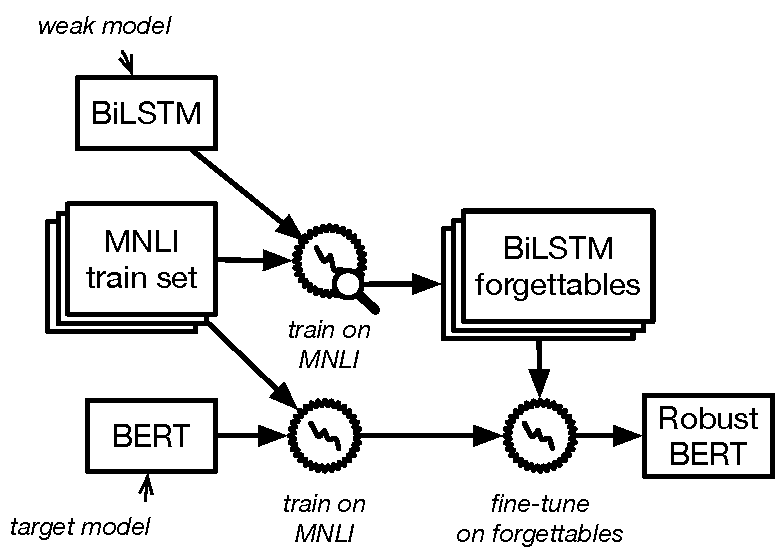
\includegraphics[scale=0.55]{figures/acl.pdf}
\caption{Proposed training for obtaining more robust natural language inference models. We first detect~\emph{forgettable}, or~\emph{hard}, examples from the MNLI training set using a weak model. These are likely to be examples that cannot be solved by simple heuristics. Then, after having fine-tuned a target model on the MNLI training set, we perform an auxiliary round of fine-tuning only on the forgettable subset to obtain a more robust model.}
\label{fig:method}
\end{figure}

\subsection{Our method}
We start from pretrained networks like BERT or XLNet.
In Fig \ref{fig:method}, the basic elements of our method is 
shown. 
We first find a set of forgettable examples using a model, 
then upweight those when training our target model by fine-tuning 
exclusively on them after fine-tuning on all examples first.

The model used for computing forgettables could be any  
simple classifier.
We do not design that model manually and since our targeted heuristics are supposed to be very common, most models' forgettables are violating those heuristics, and when we do the second stage of fine-tuning on forgettables, the target model is adapted to more challenging cases. 
Our method does not introduce a new hyperparameters and it is 
simple compared to other related work. 

To compute forgettables, we follow the original work's algorithm \cite{toneva2018empirical}
 and track the number of times each example is forgotten, following the same procedure described in \citet{toneva2018empirical}. In short, an example is forgotten if it goes from being correctly to incorrectly classified during training (because of gradient updates performed on other examples). 

If an example is forgotten at least once or is never learnt during training, we call it ``forgettable''. 
To remove the effect of shifting label distributions, we randomly sample forgettable examples for each label to keep the label distributions uniform
% of the forgettable sets identical to the ones of MNLI or QQP 
(i.e., 33\% from each of the three labels in MNLI and 50\% for the paraphrase label in QQP). 


